\chapter{Final Design}
\section{Overview}
Now that a wealth of valuable experience has been gathered through simulations and extensive testing,
a specific microphone type has been selected and an optimal array geometry for this project's use case has been identified.
This selection process was critical for achieving the project's goal of designing a fully functional, professional end product.
This chapter outlines the final design of the sound source localization system.

In the research detailed in section \ref{sec:array_prototype_measurements},
a key hypothesis emerged regarding the potential for improved sound source localization with a three-dimensional array structure as compared to a planar geometry.
This led to the development of a new mechanical concept, which is detailed later in this chapter.

For the system to function independently, it was essential to incorporate all necessary components within the design.
However, due to the computational intensity of beamforming algorithms, they cannot be processed on a microcontroller like the Teensy 4.1.
Consequently, the design had to accommodate external processing capabilities.

Another significant consideration was that a single microphone array could only provide a directional vector of located sound sources without information about the distance to these sources.
To pinpoint an object's location accurately, multiple microphone arrays are needed.
This requirement necessitated a design that allows for easy integration with a centralized computer or server, capable of connecting to multiple microphone arrays.

The optimal solution was to design a system that could stream all lossless audio data from each microphone array to the server in real-time.
Such a design ensures maximal flexibility, as it allows to apply basically any sort of localization algorithm on the server side.
In addition, it enables the usage of multiple microphone arrays, which can be placed at different locations, thus increasing the overall accuracy of the system.
\newpage

\subsection{Key Requirements}
The following key requirements have been set:
\begin{itemize}
	\item Simultaneous streaming of 32 microphone channels in real-time
	\item Lossless audio transmission with a sampling rate of 44.1\,kHz and 16\,bit resolution
	\item \acrshort{gnss} \acrshort{rtk} receiver for accurate positioning and timing information
	\item \acrshort{imu} for geographic heading and leveling information
	\item Ambient pressure and temperature sensor for calculating the exact speed of sound
	\item Ethernet interface for audio streaming and device configuration
	\item \acrshort{poe} power supply for single cable operation over long distances (up to 100\,m)
	\item Intuitive \acrfull{gui} for device configuration and monitoring
	\item Flexible mounting option for installation on a standard camera tripod
	\item Microphone integration that is resistant to the influence of wind
	\item Adjustable array arm angle for optimal beamforming performance
	\item \acrshort{rgb} \acrshort{led}s for visual feedback and status indication
\end{itemize}

\subsection{Key Decisions}
The following section describes the key decisions made during the development of the final design.
\begin{enumerate}
	\item \textbf{Microphone Type}: The \textit{MP34DT05TR-A} model by ST Microelectronics was selected for its top-ported design, offering superior audio quality and sensitivity during tests.
	\item \textbf{Microphone Integration}: To streamline the design and assembly process, dedicated \acrshort{pcb}s were designed to accommodate four microphones each.
	      This approach minimizes the need for multiple connections, as only one flex-cable is required to connect each arm to the mainboard.
	\item \textbf{Ethernet Protocol}: Given the necessity for reliable audio transmission, a \acrshort{tcp} connection was required, since a regular \acrshort{udp} connection does not guarantee packet delivery.
	\item \textbf{MCU Selection}: The \textit{Teensy 4.1} was chosen again for its proven capability in handling audio processing.
	      Its built-in 100Base-T Ethernet interface is particularly beneficial for enabling audio streaming over a \acrshort{lan} network.
	\item \textbf{GNSS Receiver}: A \acrshort{gnss} \acrshort{rtk} module from \textit{uBlox} was selected due to its high accuracy and extensive software support.
	\item \textbf{Angle Sensor}: To accurately determine the positioning of the microphone array arms, a magnetic angle sensor was used.
	      This sensor is essential for adjusting the beamforming algorithm to the current array geometry.
	\item \textbf{Mechanical Construction}: An aluminum sheet metal construction was chosen for its cost-effective manufacturing and robustness.
	\item \textbf{Touch Display}: A touch display was integrated to facilitate easy monitoring and configuration of the system.
\end{enumerate}
\newpage

\section{Mechanical Design}
Blabla


\begin{figure}[h]
	\centering
	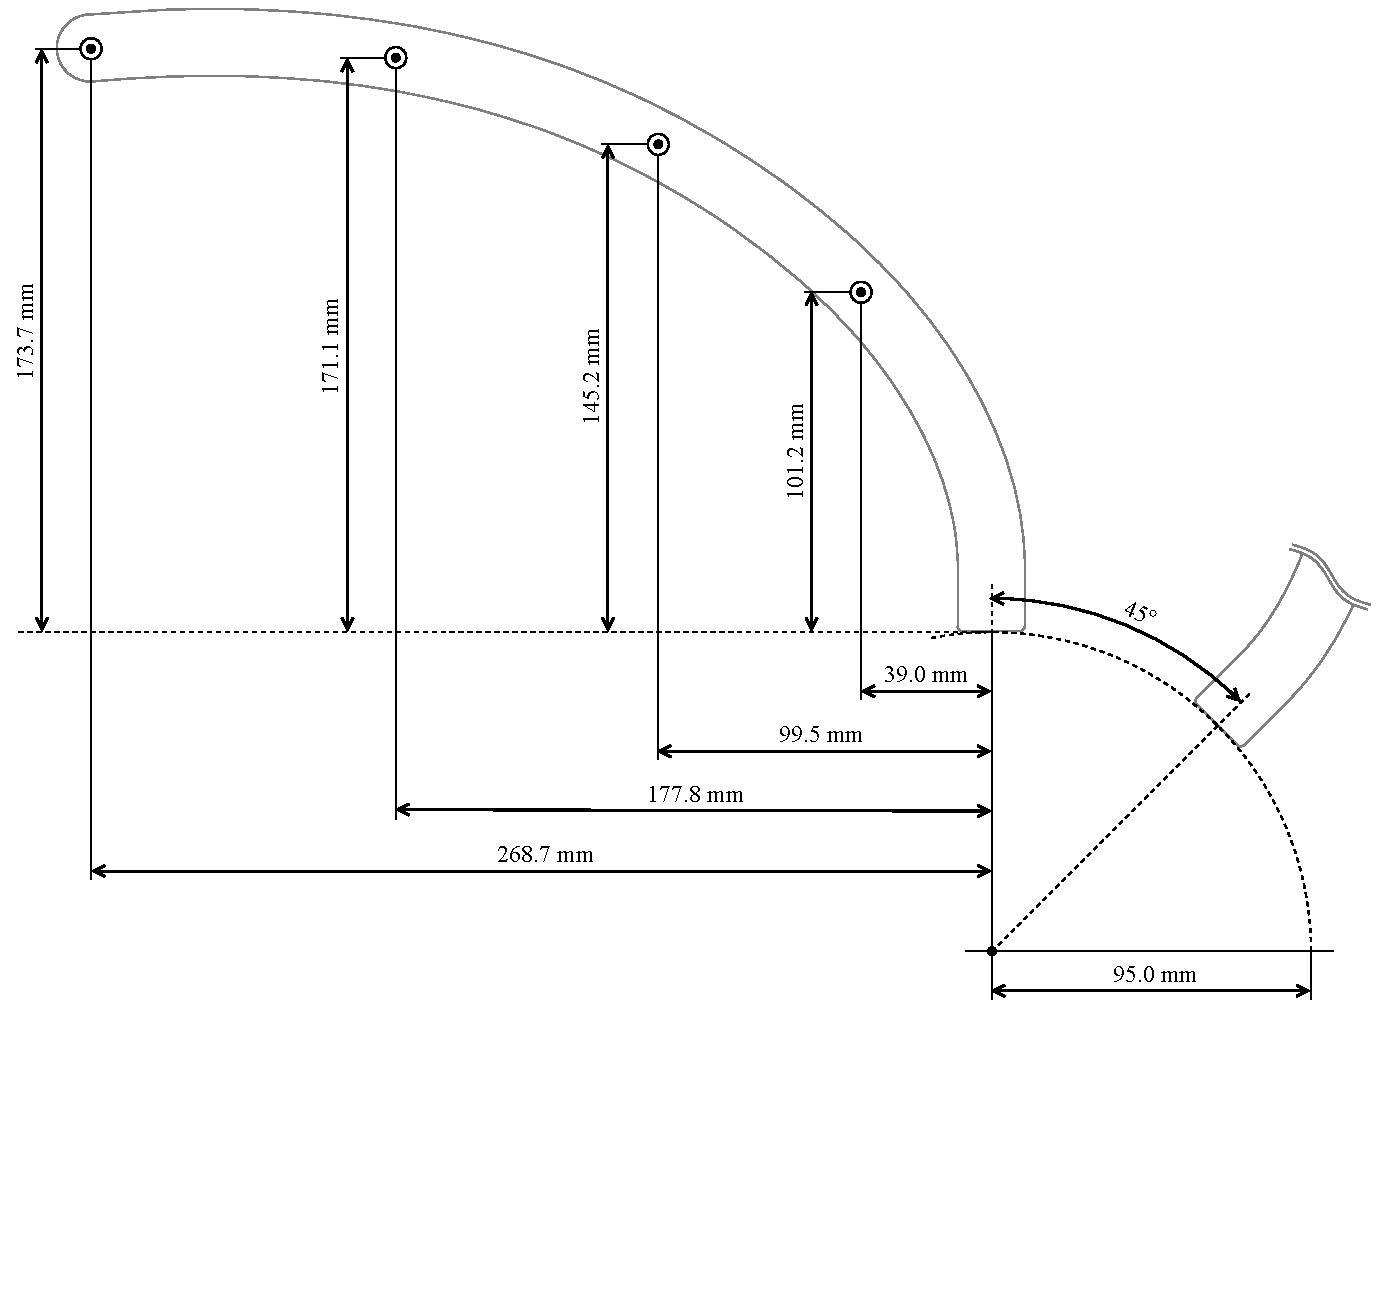
\includegraphics[width=1.0\textwidth, trim={0 4.9cm 0 0}]{images/6_design_final/array_final_design_mechanical_dimensions.pdf}
	\caption{Mechanical Dimensions of the Final Array Design}
	\label{fig:array_final_design_mechanical_dimensions}
\end{figure}


\begin{figure}[h]
	\centering
	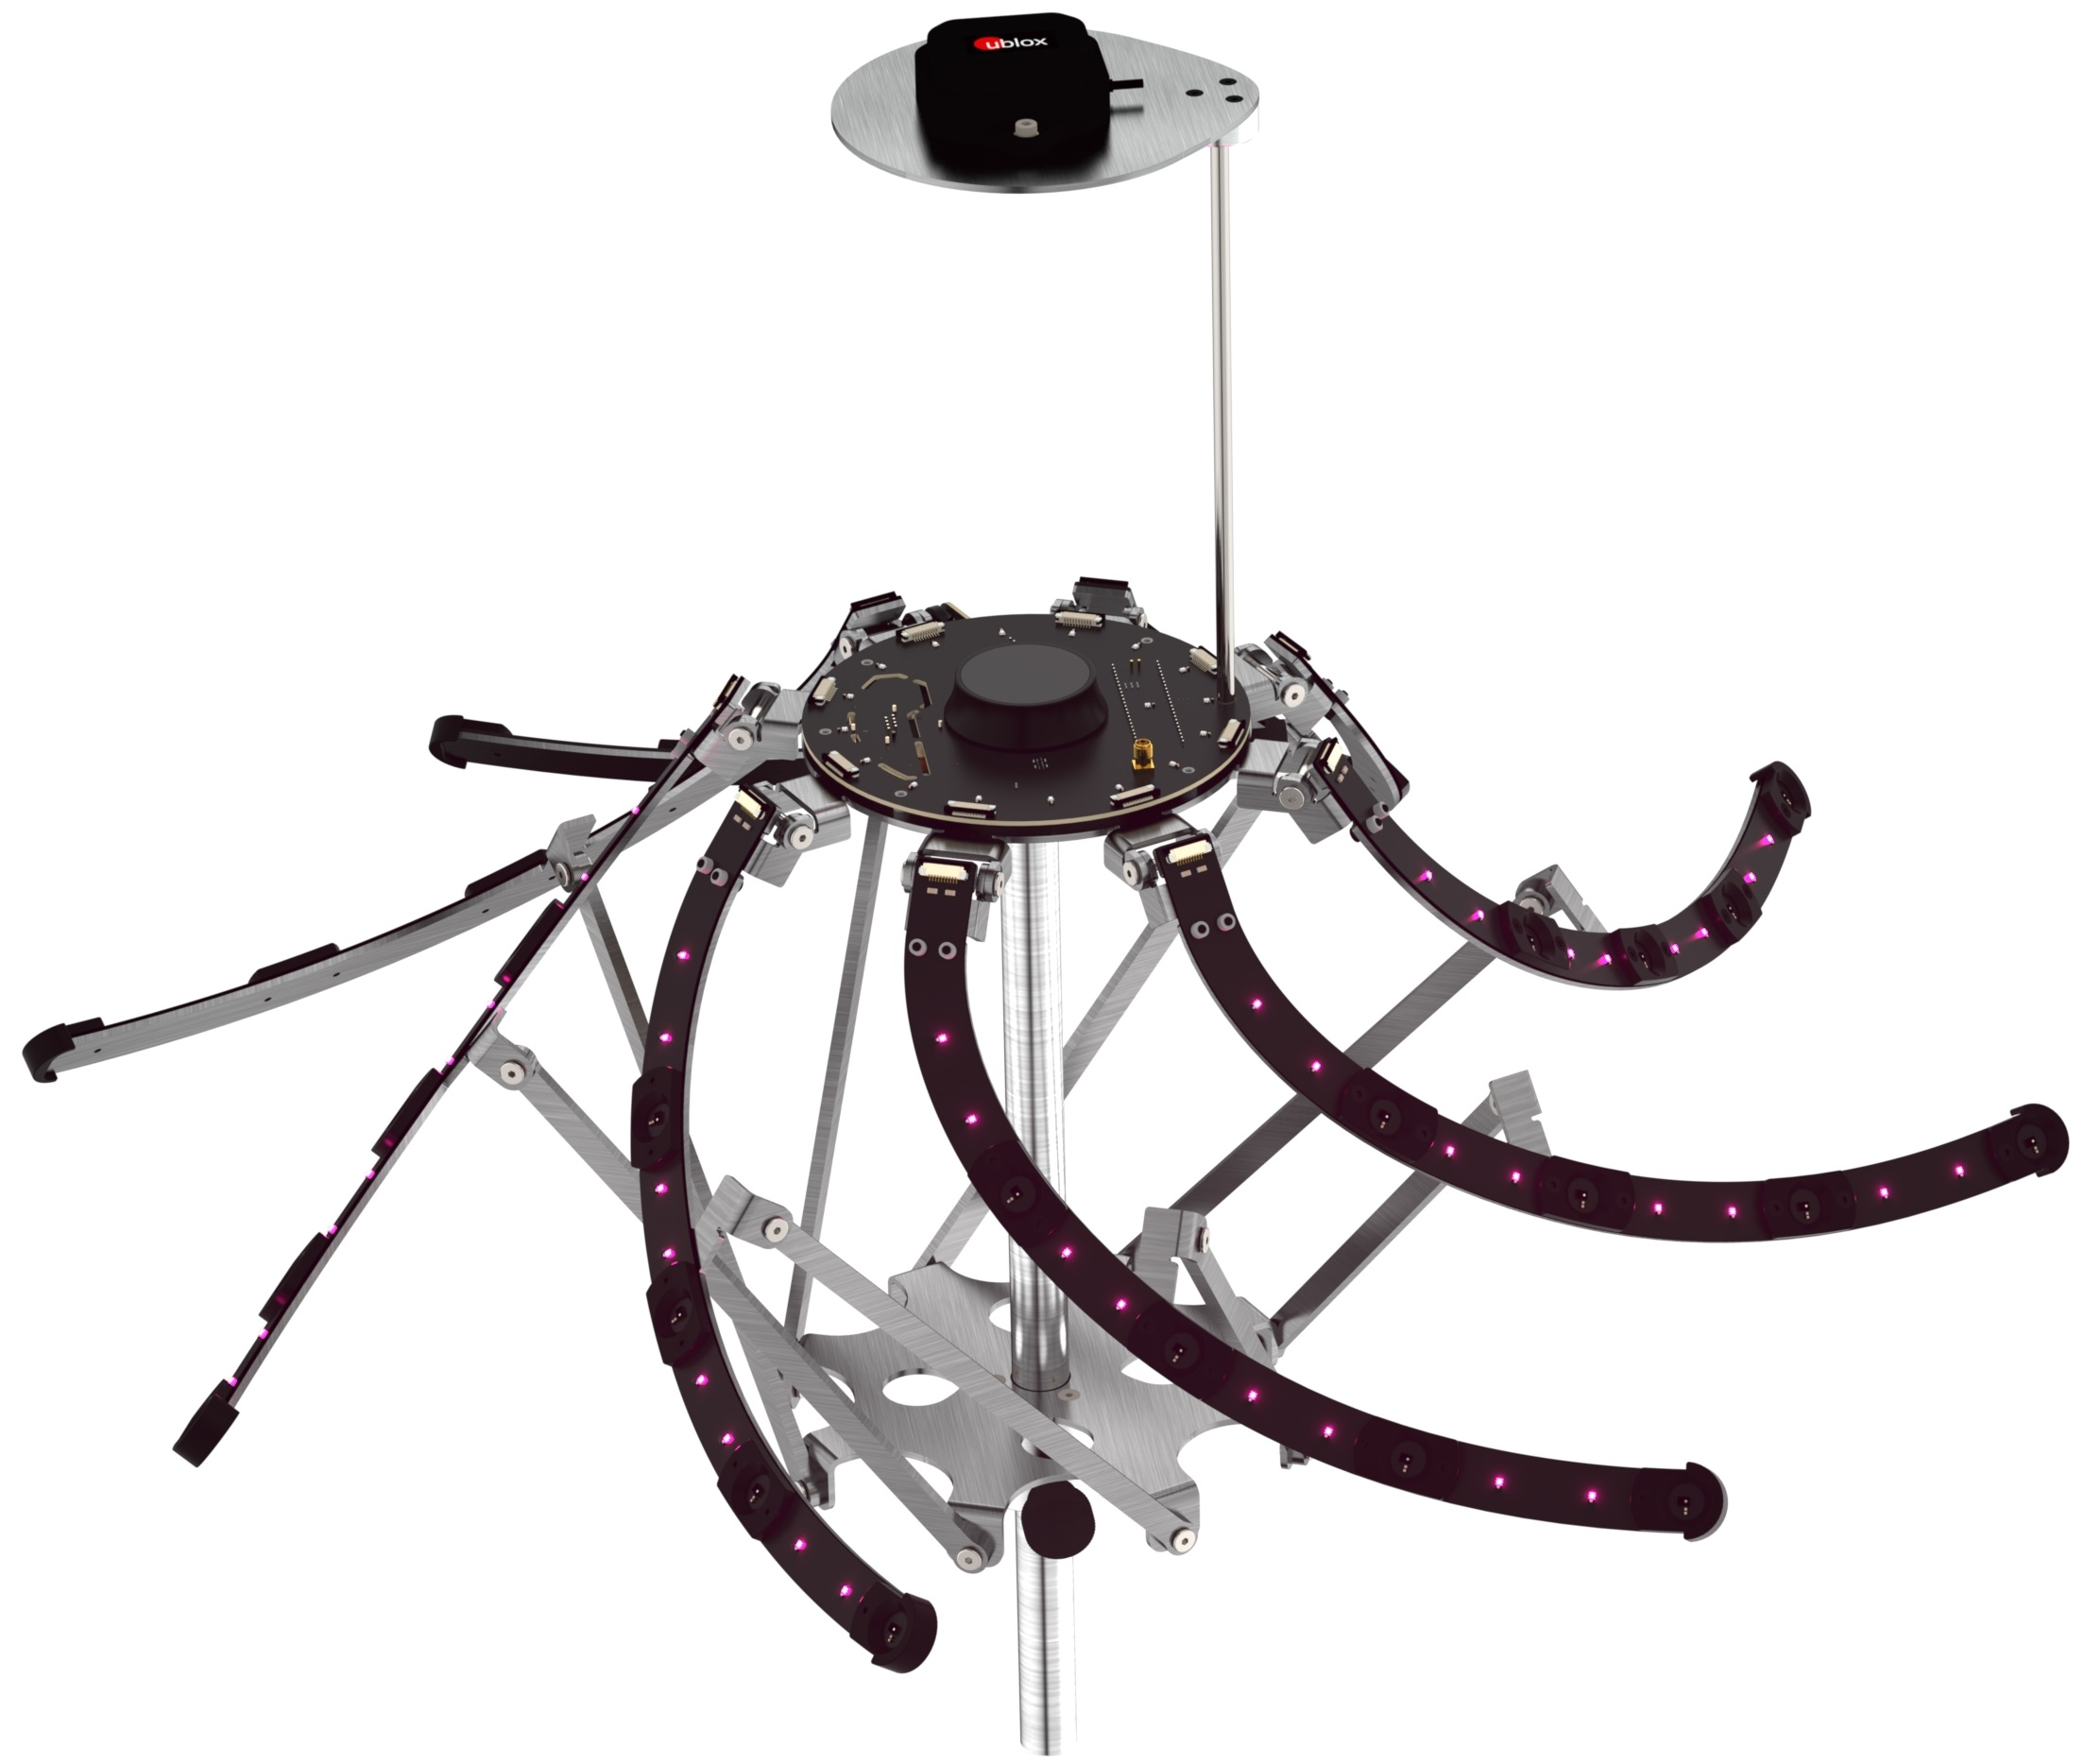
\includegraphics[width=1.0\textwidth]{images/6_design_final/final_design_3d_rendering.jpg}
	\caption{3D Rendering of the Final Design}
	\label{fig:final_design_3d_rendering}
\end{figure}




\newpage
\section{Hardware Design}
Blabla
\begin{figure}[h]
	\centering
	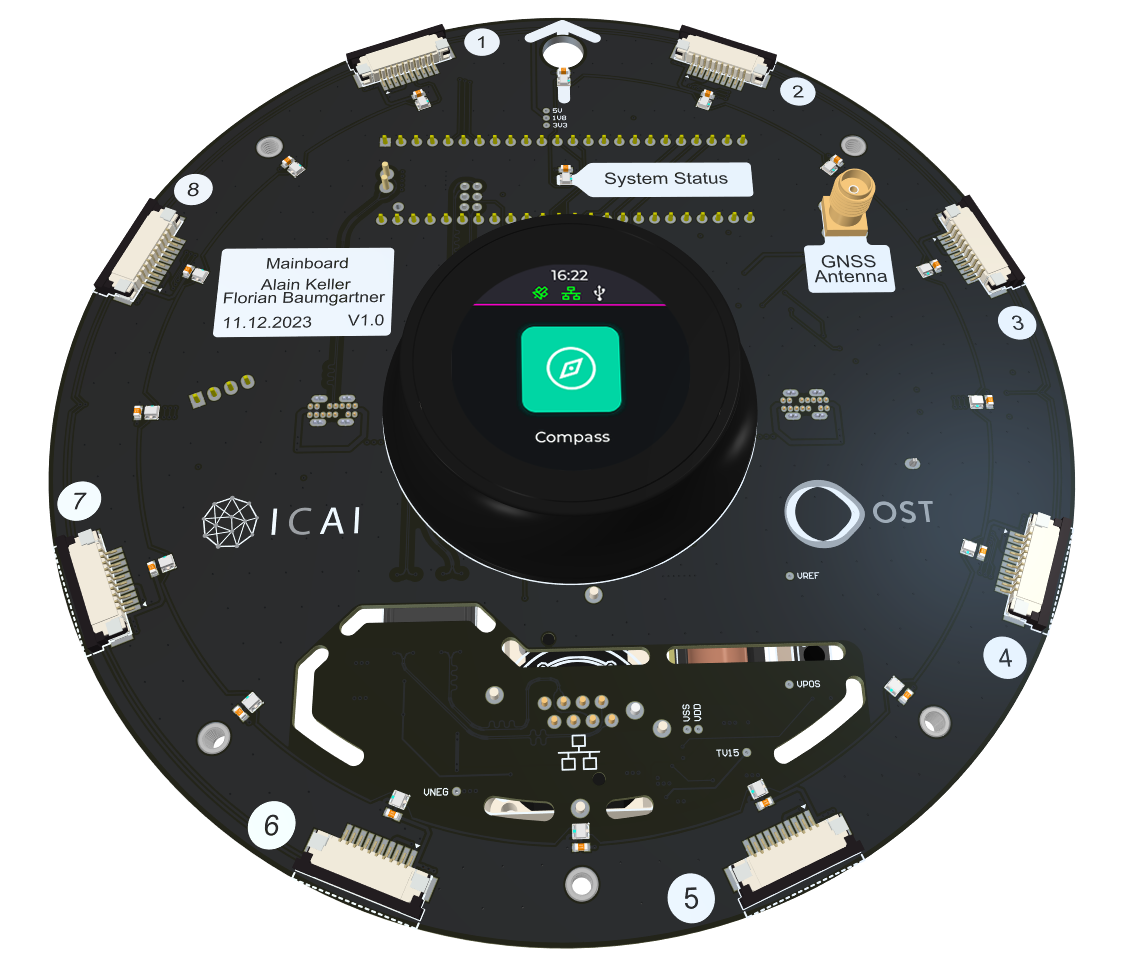
\includegraphics[width=1.0\textwidth]{images/6_design_final/Mainboard_Front_Display.png}
	\caption{Front view of the mainboard}
	\label{fig:mainboard_front}
\end{figure}
\newpage



\subsection{Block Diagram}
\begin{figure}[h]
	\centering
	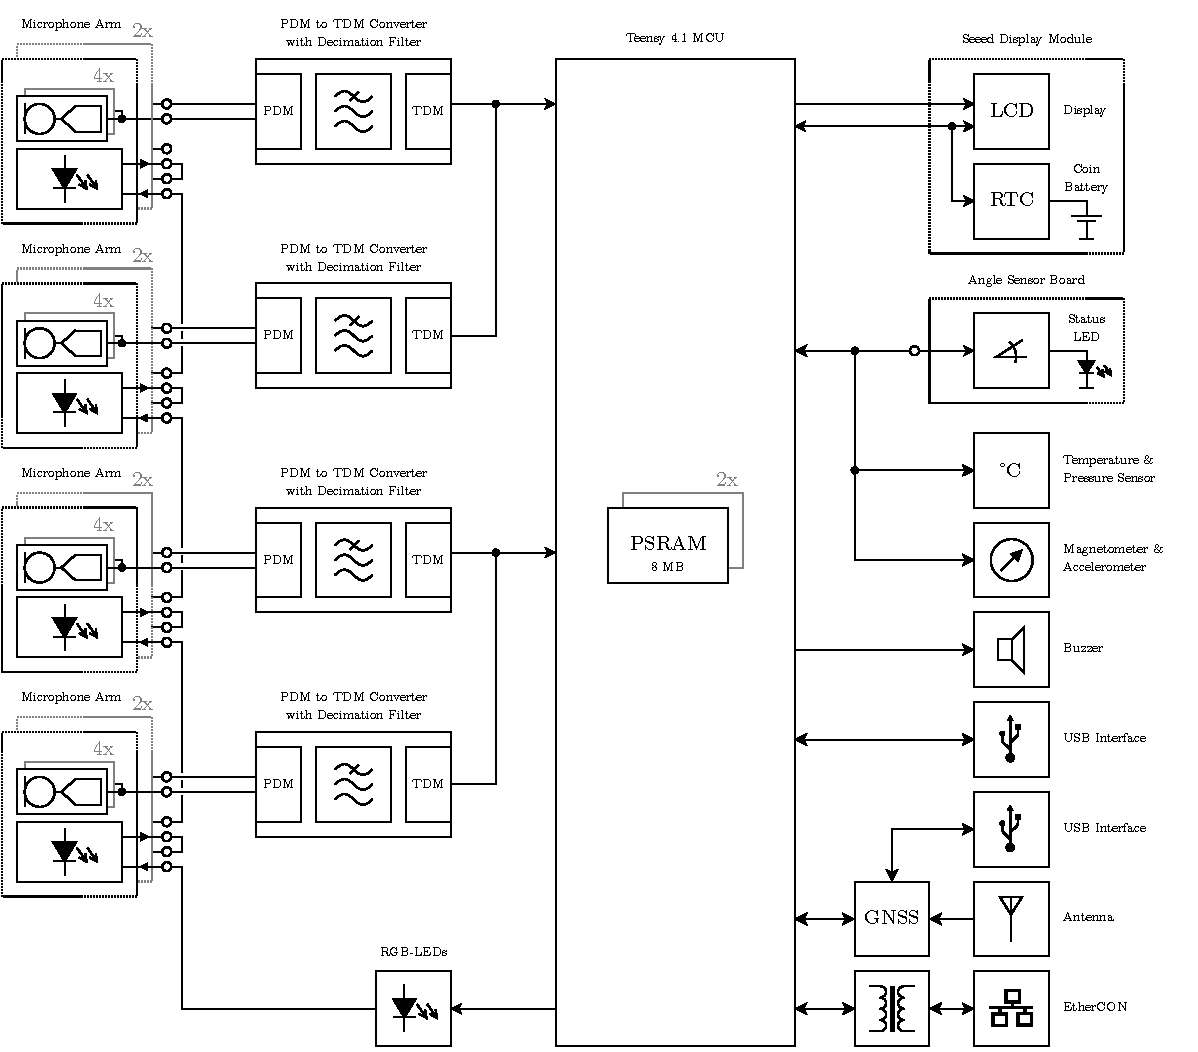
\includegraphics[width=1.0\textwidth, trim={0 0 0.5cm 0}]{images/6_design_final/final_design_block_diagram.pdf}
	\caption{System block diagram}
	\label{fig:system_block_diagram}
\end{figure}

\subsection{Power Supply}
The device can be powered by multiple sources. Primary the device is powered by the ethernet interface, which provides a \acrfull{poe} connection.
This is the preferred method, as it is the most convenient way to use the microphone array in the field.
In addition, there are two USB-C ports (\acrshort{mcu} and \acrshort{gnss}) that can be used to supply power when no PoE connection is available (e.g. in a laboratory environment for programming and debugging).
Each supply method can be used in conjunction with each other. However, the source must be able to provide at least 12.5\,W of power (5\,V, 2.5\,A).
In figure \ref{fig:power_supply_overview} an overview of the power supply is shown.
Note that the Teensy 4.1 has an internal 3.3\,V regulator, which is powered by the systems internal 5\,V supply.
The 1.8\,V rail is generated by a dedicated linear voltage regulator and is mainly used for the \acrshort{pdm} to \acrshort{tdm} converters (ADAU7118).

\begin{figure}
	\centering
	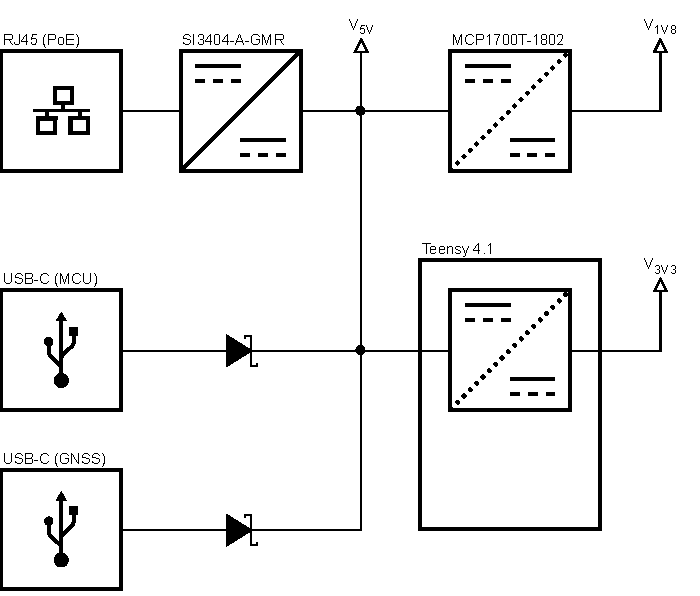
\includegraphics[width=0.65\textwidth]{images/6_design_final/final_design_power_supply.pdf}
	\caption{Power Supply Overview}
	\label{fig:power_supply_overview}
\end{figure}

\subsubsection{Power over Ethernet (PoE)}


\subsection{Microcontroller Unit (MCU)}

%  TODO: Write about external PSRAM

\subsection{Audio Input}

\subsection{GNSS}

\subsection{Human Machine Interface (HMI)}

%  TODO: Wite about LEDs and Buzzer

\subsection{LCD Display}

\subsection{RGB LEDs}

\subsection{Sensors}

\subsubsection{Magnetometer \& Accelerometer Sensor}

\subsubsection{Ambient Pressure \& Temperature Sensor}

\subsubsection{Angle Sensor}

\subsection{Printed Circuit Board (PCB)}

\subsubsection{Mainboard}

\subsubsection{Microphone Arms}

\subsubsection{Angle Sensor}

\subsection{Manufacturing}
The PCBs were manufactured and assembled by JLCPCB.
Only a few additional components were soldered by hand, such as the PDM to TDP converters (ADAU7118), the EtherCon connector and the GNSS module (NEO-M8P-2).
It turned out that multiple microphone arm PCBs were faulty (damaged microphones).
This was most likely caused by the soldering process, as the MEMS microphones are very sensitive to heat.

\newpage
\section{Firmware Design}
Blabla

\subsection{Overview}

\begin{table}[h]
	\centering
	\begin{tabular}{|l|l|}
		\hline
		Thread                     & Purpose                      \\ \hline
		\texttt{Console Interface} & Handles USB virtual COM-Port \\ \hline
		\texttt{Console Streaming} & Handles queuing of messages  \\ \hline
		\texttt{Utils}             & Updates operation time       \\ \hline
		\texttt{AudioUtils}        & Audio Processing             \\ \hline
		\texttt{GNSS}              & GNSS Data Handling           \\ \hline
		\texttt{HMI}               & LED Control \& RTC           \\ \hline
		\texttt{Buzzer}            & Buzzer Control               \\ \hline
		\texttt{Application}       & Main Application Logic       \\ \hline
		\texttt{Main}              & Main Thread (Background)     \\ \hline
	\end{tabular}
	\caption{Overview of all threads and their purpose}
	\label{tab:threads}
\end{table}


\subsection{Audio Streaming}
The audio streaming module handles the buffering and transmission of the 32 audio channels.
It is based on a TCP server that provides a socket connection on port 6666.
The audio data is transmitted in a lossless 16-bit signed integer format, with a sample rate of 44.1 kHz.

The TCP connection asures a reliable data transmission, which is essential for the audio data.
To provide a low latency audio stream, the audio data is buffered in a circular buffer of 12 MB size.
This allows for a maximum delay of ca. 4.4\,s.

For a continuous audio stream, a tranmission rate of
\begin{equation}
	\frac{32\,\text{channels} \cdot 16\,\text{bit} \cdot 44100\,\text{Hz}}{10^6\,\text{bit/s}} = 22.1184\,\text{Mbit/s}
\end{equation}
is required.
The theoretical maximum transmission rate of 100Base-T Ethernet is 100\,Mbit/s.
However, the maximum transmission rate of the Teensy 4.1 is around 60\,Mbit/s, which is still sufficient for the audio stream.

Due to the maximal TCP packet size of 1460 bytes, the audio data is split into concatenated packets.
A frame consists of 128 interleafed samples (32 channels) and is transmitted in 8 packets.
Each frame starts with a 20-byte header.

\begin{table}[h]
	\centering
	\begin{tabular}{|l|l|l|l|}
		\hline
		\textbf{Byte Offset} & \textbf{Data Format}    & \textbf{Description} & \textbf{Example Value} \\ \hline
		0-7                  & String                  & Magic Sequence       & \codeword{HERON666}    \\ \hline
		8-11                 & Integer (Little Endian) & Packet Index         & 12345                  \\ \hline
		12-19                & Integer (Little Endian) & Timestamp (ns)       & 1713586842696942069    \\ \hline
	\end{tabular}
	\caption{Description of the 20-byte Packet Header}
	\label{tab:packet_header}
\end{table}

\begin{figure}[h]
	\centering
	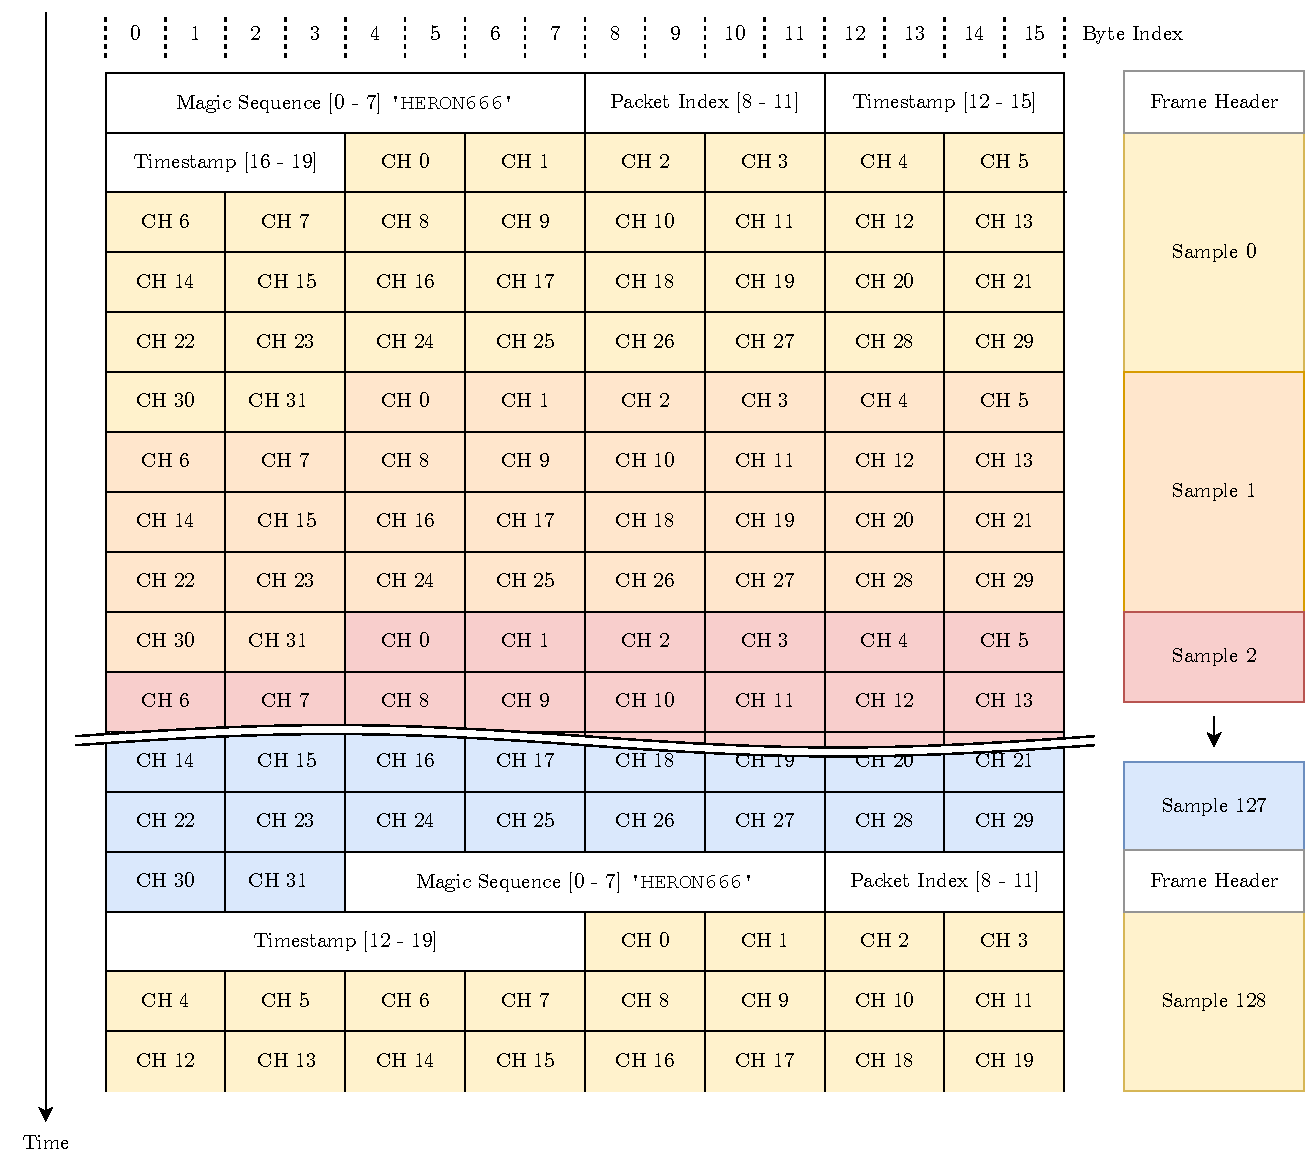
\includegraphics[width=1.0\textwidth]{images/6_design_final/Audio_Stream_Frame.pdf}
	\caption{Example of a Frame with 128 Samples (32 Channels)}
	\label{fig:frame_example}
\end{figure}

\subsection{GNSS \& RTC Time}

\subsubsection{GNSS Time}

\subsubsection{RTC Time}

\subsubsection{Phased Locked Loop (PLL)}

\subsubsection{Remote Configuration}
The

\begin{table}[h]
	\tiny
	\centering
	\begin{tabular}{|l|l|l|l|l|}
		\hline
		\textbf{Data Field}         & \textbf{Description}          & \textbf{Data Type} & \textbf{Unit} & \textbf{Example Value} \\ \hline
		device\_firmware\_version   & Firmware Version              & String             & -             & "V0.1"                 \\ \hline
		device\_firmware\_build     & Firmware Build Date           & String             & -             & "240110"               \\ \hline
		device\_cpu\_frequency      & CPU Frequency                 & Integer            & Hz            & 912000000              \\ \hline
		device\_cpu\_temperature    & Current CPU Temperature       & Float              & °C            & 36.5                   \\ \hline
		device\_operating\_time     & Device Operating Time         & Integer            & s             & 15615                  \\ \hline
		device\_system\_warning     & Current System Warning Status & Boolean            & -             & false                  \\ \hline
		ethernet\_mac               & MAC Address                   & String             & -             & "48:53:52:20:3C:33"    \\ \hline
		ethernet\_ip                & Current IP Address            & String             & -             & "192.168.1.10"         \\ \hline
		streaming\_state            & Current Streaming State       & Boolean            & -             & true                   \\ \hline
		streaming\_speed            & Current Streaming Speed       & Float              & Mbit/s        & 22.21                  \\ \hline
		streaming\_buffer           & Streaming Buffer Fill Level   & Float              & \%            & 15.1                   \\ \hline
		sensor\_heading             & Device Heading                & Float              & °             & 270.0                  \\ \hline
		sensor\_pitch               & Device Pitch                  & Float              & °             & 5.2                    \\ \hline
		sensor\_roll                & Device Roll                   & Float              & °             & 2.4                    \\ \hline
		sensor\_temperature         & Ambient Temperature           & Float              & °C            & 22.3                   \\ \hline
		sensor\_pressure            & Ambient Pressure              & Float              & hPa           & 1013.2                 \\ \hline
		sensor\_altitude            & Device Altitude               & Float              & m (MSL)       & 434.5                  \\ \hline
		sensor\_angle               & Arm Angle                     & Float              & °             & 45.7                   \\ \hline
		sensor\_magnet\_detected    & Magnet Detection Status       & Boolean            & -             & true                   \\ \hline
		sensor\_magnet\_too\_weak   & Magnet Too Weak Status        & Boolean            & -             & false                  \\ \hline
		sensor\_magnet\_too\_strong & Magnet Too Strong Status      & Boolean            & -             & false                  \\ \hline
		gnss\_latitude              & GNSS Latitude                 & Float              & °             & 40.7128                \\ \hline
		gnss\_longitude             & GNSS Longitude                & Float              & °             & -74.0060               \\ \hline
		gnss\_altitude              & GNSS Altitude                 & Float              & m (MSL)       & 344.8                  \\ \hline
		gnss\_magnetic\_declination & GNSS Magnetic Declination     & Float              & °             & -5.0                   \\ \hline
		gnss\_satelite\_count       & GNSS Satellite Count          & Integer            & -             & 8                      \\ \hline
		gnss\_fix                   & GNSS Fix Status               & Boolean            & -             & true                   \\ \hline
		gnss\_fix\_type             & GNSS Fix Type                 & Integer            & -             & 3                      \\ \hline
		gnss\_time\_valid           & GNSS Time Validity            & Integer            & UNIX (UTC+0)  & 1704921651             \\ \hline
	\end{tabular}
	\caption{Device Data JSON File Fields, Descriptions, Data Types, Units, and Example Values}
	\label{table:device_data_types}
\end{table}


For remote configuration, the client (e.g. a PC) sends a JSON file containing the desired command and its parameters to the device.

\begin{table}[h]
	\tiny
	\centering
	\begin{tabular}{|l|l|l|l|l|}
		\hline
		\textbf{Data Field}    & \textbf{Description}                       & \textbf{Data Type} & \textbf{Unit} & \textbf{Example Value} \\ \hline
		clear\_warning         & Clears the warning status                  & Boolean            & -             & true / false           \\ \hline
		gnss\_coefficient\_xxx & GNSS RTK Coefficient XXX (Not implemented) & Float              & -             & -                      \\ \hline
	\end{tabular}
	\caption{Overview of Received Commands in JSON File}
	\label{tab:received_commands}
\end{table}

\subsection{Sensor Calibration}


\clearpage
\subsection{Graphical User Interface (GUI)}
The GUI provides a user-friendly interface for configuring the device and monitoring its status.
It is based on the LVGL framework.



\clearpage
\subsection{GUI Pages}
In the following sections, the different GUI pages are explained in detail.
Navigating between the pages is done by clicking on the corresponding icon in the home menu.
To return to the home menu, the sub-page header bar with the arrow symbol can be pressed.
Figure \ref{fig:gui_pages_overview} shows an overview of all GUI pages and how navigation between them is done.
\begin{figure}[h]
	\centering
	\vspace{-0.5cm}
	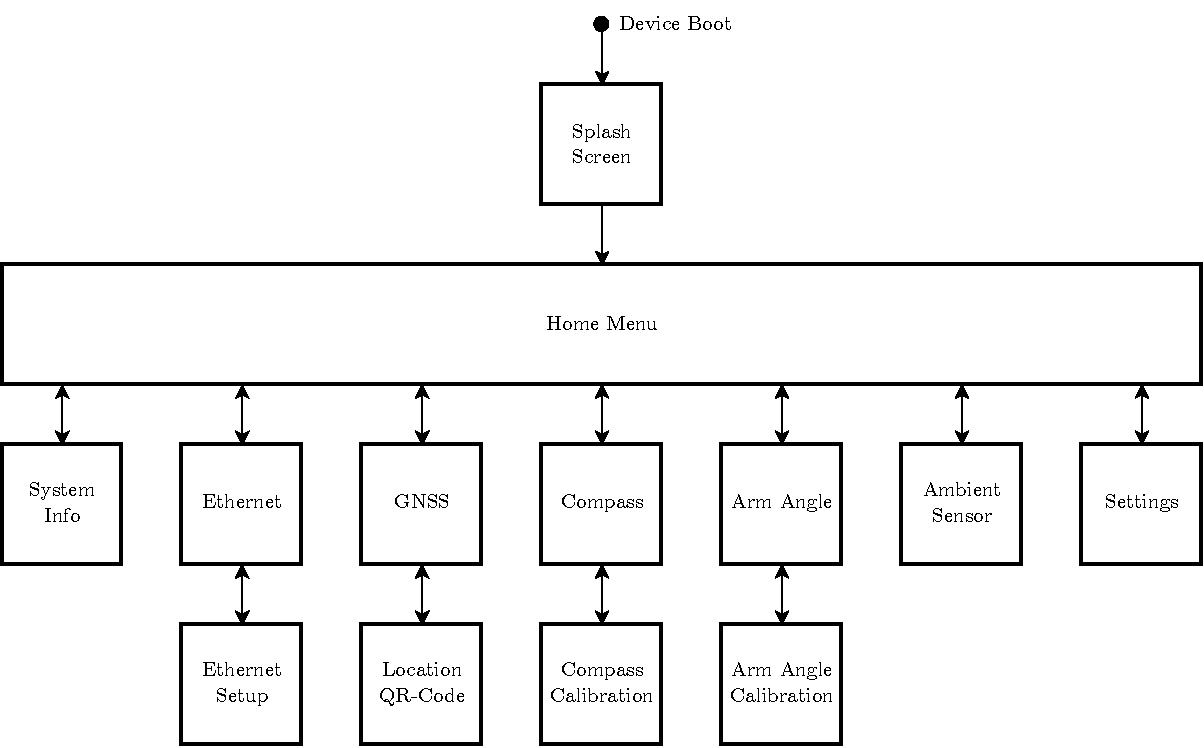
\includegraphics[width=0.85\textwidth]{images/6_design_final/final_design_gui_pages.pdf}
	\caption{GUI Pages Overview}
	\label{fig:gui_pages_overview}
\end{figure}
\vspace{-0.3cm}

\begin{minipage}{\linewidth}
	\begin{wrapfigure}{l}{4.5cm}
		\vspace{-0.6cm}
		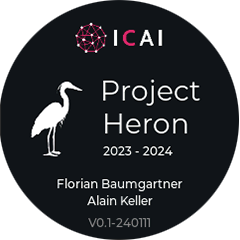
\includegraphics[width=4cm]{images/6_design_final/gui/00_splash_screen.png}
		\centering
		\caption{Splash Screen}
		\label{fig:final_design_gui_splash_screen}
	\end{wrapfigure}
	\subsubsection{Splash Screen}
	When the system is powered on, the splash screen is displayed for 5 seconds.
	On the bottom of the screen, the current firmware version and build date is displayed.
	After the system has booted, the home menu is displayed.
\end{minipage}
\vspace{2.2cm}		% One line corresponds to ca. 0.4cm

\begin{minipage}{\linewidth}
	\begin{wrapfigure}{l}{4.5cm}
		\vspace{-0.6cm}
		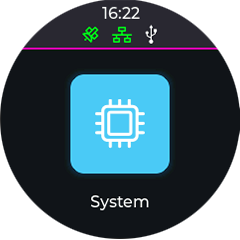
\includegraphics[width=4cm]{images/6_design_final/gui/01_main_menu.png}
		\centering
		\caption{Home Menu}
		\label{fig:final_design_gui_home_menu}
	\end{wrapfigure}
	\subsubsection{Home Menu}
	The home menu presents an intuitive way of navigating through the different submenus.
	On the top of the screen, the current time is displayed.
	A dedicated icon for the \acrshort{gnss}, ethernet and \acrshort{usb} interface is shown.
	Per default, the icons are grayed out.
	When the \acrshort{gnss} location is valid (fix), the icon turns green.
	When the device is connected to the network but is not yet streaming, the icon is filled white.
	As soon as the audio stream is active, the icon turns green.
	The \acrshort{usb} icon is filled white when a device is connected to the \acrshort{usb} port.
	As soon as the virtual COM port is opened, the icon turns green.
\end{minipage}
\pagebreak

\begin{minipage}{\linewidth}
	\begin{wrapfigure}{l}{4.5cm}
		\vspace{-0.6cm}
		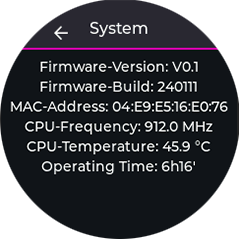
\includegraphics[width=4cm]{images/6_design_final/gui/03_system_info.png}
		\centering
		\caption{System Information}
		\label{fig:final_design_gui_system_info}
	\end{wrapfigure}
	\subsubsection{System Information}
	The system information page displays important device information such as the firmware version,
	firmware build date, etherent \acrshort{mac} address, \acrshort{cpu} frequency and temperature, as well as the operating time.
\end{minipage}
\vspace{1.3cm}

\begin{minipage}{\linewidth}
	\begin{wrapfigure}{l}{4.5cm}
		\vspace{-0.6cm}
		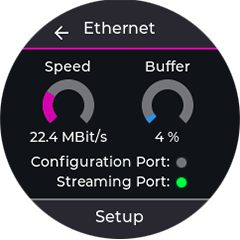
\includegraphics[width=4cm]{images/6_design_final/gui/04_ethernet.png}
		\centering
		\caption{Ethernet}
		\label{fig:final_design_gui_ethernet}
	\end{wrapfigure}
	\subsubsection{Ethernet}
	The ethernet page displays the current connection state of the streaming and configuration port.
	While a connection is established to either of the ports, the corresponding gray circle is filled green.
	Two gauge bars display the current streaming speed and the fill level of the streaming buffer.
	In normal operation, the indicated streaming speed should be around 22\,Mbit/s and the buffer fill level near 0\,\%.
\end{minipage}
\vspace{0.0cm}

\begin{minipage}{\linewidth}
	\begin{wrapfigure}{l}{4.5cm}
		\vspace{-0.6cm}
		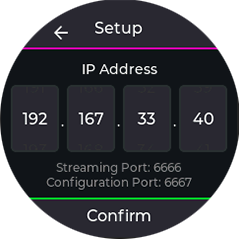
\includegraphics[width=4cm]{images/6_design_final/gui/05_ethernet_config.png}
		\centering
		\caption{Ethernet Setup}
		\label{fig:final_design_gui_ethernet_setup}
	\end{wrapfigure}
	\subsubsection{Ethernet Setup}
	The ethernet setup page allows for configuring the \acrshort{ip} address  of the device.
	Below the \acrshort{ip} address, the hard-coded streaming port (6666) and configuration port (6667) is displayed.
	When the \acrshort{ip} address is changed, the user can either confirm the change or discard it by returning to the previous page.
	When a new \acrshort{ip} address is confirmed, the device will instantly change its \acrshort{ip} address and restart the servers.
\end{minipage}
\vspace{0.0cm}

\begin{minipage}{\linewidth}
	\begin{wrapfigure}{l}{4.5cm}
		\vspace{-0.6cm}
		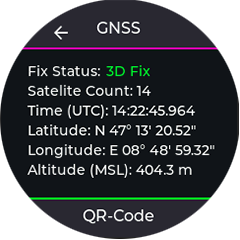
\includegraphics[width=4cm]{images/6_design_final/gui/06_gnss.png}
		\centering
		\caption{GNSS}
		\label{fig:final_design_gui_gnss}
	\end{wrapfigure}
	\subsubsection{GNSS}
	The \acrshort{gnss} page displays the current status of the \acrshort{gnss} module.
	When the Fix Status is valid (2D-Fix or 3D-Fix), the latitude, longitude and altitude is displayed.
	In addition, the QR-Code button gets enabled, which allows for displaying the current location in a QR-Code.
	The coordinates are displayed in degrees, minutes and seconds.
	The altitude is displayed in meters above sea level (MSL).
	When the time is fully resolved, it is displayed in the UTC+0 format.
	While the Fix Status is invalid, all fields are grayed out.
\end{minipage}
\vspace{0.0cm}

\begin{minipage}{\linewidth}
	\begin{wrapfigure}{l}{4.5cm}
		\vspace{-0.6cm}
		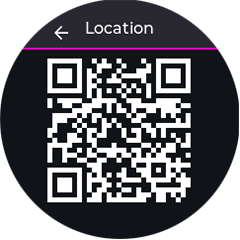
\includegraphics[width=4cm]{images/6_design_final/gui/07_gnss_location.png}
		\centering
		\caption{Location QR-Code}
		\label{fig:final_design_gui_gnss_location}
	\end{wrapfigure}
	\subsubsection{GNSS Location QR-Code}
	The \acrshort{gnss} location \acrshort{qr}-Code page displays a \acrshort{qr}-Code containing a google maps link to the current location.
	When the \acrshort{qr}-Code is scanned with a smartphone, the web broweser will immediately redirect the user to the google maps app.
	The \acrshort{url} is formated as follows: \smallskip \newline
	\codeword{google.com/maps/place/<latitude>,<longitude>} \smallskip \newline
	For example, the \acrshort{url} directs to: \smallskip \newline
	\url{google.com/maps/place/47.222400,8.816460}
\end{minipage}
\vspace{-0.2cm}

\begin{minipage}{\linewidth}
	\begin{wrapfigure}{l}{4.5cm}
		\vspace{-0.6cm}
		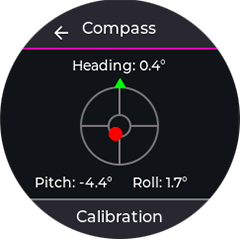
\includegraphics[width=4cm]{images/6_design_final/gui/08_compass.png}
		\centering
		\caption{Compass}
		\label{fig:final_design_gui_compass}
	\end{wrapfigure}
	\subsubsection{Compass}
	The compass page displays the current heading and leveling of the device.
	The heading is indicated by a purple arrow, pointing towards geographic north.
	When the needle points exactly towards the top of the screen it turns green, meaning the device is facing north.
	The circular graphic in the centre of the screen shows the current leveling of the device.
	When the device is perfectly leveled, the circle turns green.
	When the device is tilted, the circle turns red and the tilt angle is displayed in degrees (pitch and roll).
	To calibrate the built-in magnetometer, the user can press the calibrate button.
\end{minipage}
\vspace{-0.2cm}

\begin{minipage}{\linewidth}
	\begin{wrapfigure}{l}{4.5cm}
		\vspace{-0.6cm}
		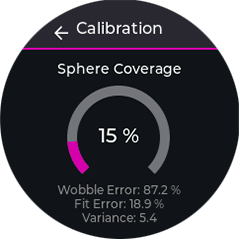
\includegraphics[width=4cm]{images/6_design_final/gui/09_compass_calibration.png}
		\centering
		\caption{Compass Calib.}
		\label{fig:final_design_gui_compass_calibration}
	\end{wrapfigure}
	\subsubsection{Compass Calibration}
	The compass calibration page displays the current status of the magnetometer calibration.
	By entering this page, the calibration process is starts immediately.
	To calibrate the magnetometer, the device has to be rotated around all three axes.
	This process takes around 30 seconds.
	As soon as the spere coverage indicator reaches 100\,\%, the calibration is finished, a success message is displayed and the buzzer plays a short melody.
	The calibration process can be aborted at any time by returning to the previous page (the calibration progress is not saved).
\end{minipage}
\vspace{-0.2cm}

\begin{minipage}{\linewidth}
	\begin{wrapfigure}{l}{4.5cm}
		\vspace{-0.6cm}
		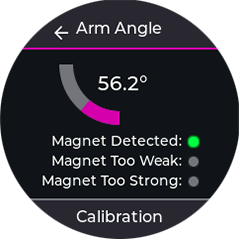
\includegraphics[width=4cm]{images/6_design_final/gui/10_angle_sensor.png}
		\centering
		\caption{Arm Angle}
		\label{fig:final_design_gui_arm_angle}
	\end{wrapfigure}
	\subsubsection{Arm Angle}
	The arm angle page displays the current angle of the microphone array arms in degree.
	When the arms are fully unfolded (horizontal) the angle is 0.0\,°.
	When the arms are fully folded towards the centre pole the angle is 90.0\,°.
	Below the angle indicator, the current status of the magnet detection is displayed.
	When the magnet is detected, the status indicator turns green.
	If the magnet is too weak or too strong, the corresponding status indicator turns yellow.
	Otherwise, the status indicators are grayed out.
\end{minipage}
\pagebreak

\begin{minipage}{\linewidth}
	\begin{wrapfigure}{l}{4.5cm}
		\vspace{-0.6cm}
		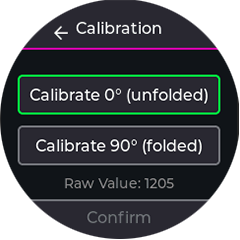
\includegraphics[width=4cm]{images/6_design_final/gui/11_angle_sensor_calibration.png}
		\centering
		\caption{Arm Angle Calib.}
		\label{fig:final_design_gui_arm_angle_calibration}
	\end{wrapfigure}
	\subsubsection{Arm Angle}
	The arm angle calibration page lets the user calibrate the angle sensor.
	To calibrate the angle sensor, the arms have to be fully unfolded (horizontal).
	Then the upper calibrate button \textit{Calibrate 0° (unfolded)} has to be pressed.
	Next, the arms have to be fully folded towards the centre pole.
	Then the lower calibrate button \textit{Calibrate 90° (folded)} has to be pressed.
	To confirm the calibration, the user has to press the \textit{Confirm} button.
\end{minipage}
\vspace{0.0cm}

\begin{minipage}{\linewidth}
	\begin{wrapfigure}{l}{4.5cm}
		\vspace{-0.6cm}
		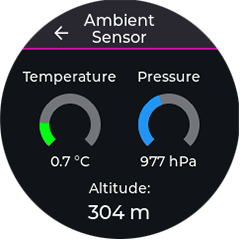
\includegraphics[width=4cm]{images/6_design_final/gui/12_ambient_sensor.png}
		\centering
		\caption{Ambient Sensor}
		\label{fig:final_design_gui_ambient_sensor}
	\end{wrapfigure}
	\subsubsection{Ambient Sensor}
	The ambient sensor page displays the current ambient temperature in degree Celsius and the ambient pressure in hectopascal.
	A gauge bar visualizes both values.
	Based on the current ambient pressure, the altitude above sea level is calculated and displayed in meters.
	Note that the altitude is only an approximation and can be inaccurate.
	It is strongly influenced by the current weather conditions.
\end{minipage}
\vspace{0.5cm}

\begin{minipage}{\linewidth}
	\begin{wrapfigure}{l}{4.5cm}
		\vspace{-0.6cm}
		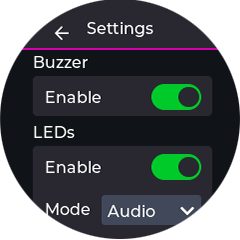
\includegraphics[width=4cm, trim={0 -1.0cm 0 0}]{images/6_design_final/gui/13_settings.png}
		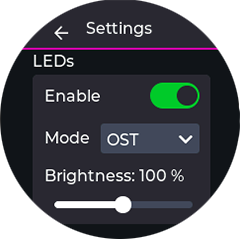
\includegraphics[width=4cm]{images/6_design_final/gui/14_settings.png}
		\centering
		\caption{Settings}
		\label{fig:final_design_gui_settings}
	\end{wrapfigure}
	\subsubsection{Settings}
	The settings page allows the user to configure the device.
	First, the buzzer can be enabled or disabled.
	Second, the \acrshort{led}s can be permanently enabled or disabled.
	The mode selection provides a selection of different animations for the \acrshort{led}s.
	Currently, there are two animation types implemented:
	\begin{itemize}
		\setlength{\itemindent}{5mm}
		\setlength{\leftmargin}{10mm}
		\item \textbf{Audio:} The \acrshort{led}s are controlled by the audio level of the microphone array.
		\item \textbf{OST:} The \acrshort{led}s show a fluent animation in the \acrshort{ost} color scheme.
	\end{itemize}
	Below the mode settings, the \acrshort{led} brightness can be adjusted.
	All settings are saved in the internal flash memory of the device and are restored after a reboot.
\end{minipage}


\newpage
\section{Software Design}
Blabla




